%!TEX root = ../../lod-group1.tex
\subsection{Updating}
\label{subsec_evaluation_updating}

The scheduler, described in Chapter \ref{subsec_method_updating}, updates movies at certain times.
Thereby, the scheduler distinguishes between existing and upcoming movies.

The amount of upcoming movies which are added to IMDb every day is shown in Figure \ref{fig_coming_soon_movie}.
On a daily basis, the coming soon page of IMDb was crawled and the changes were recorded.
Almost every day, new movies are added or deleted from the IMDb coming soon list.
It is noticeable, that most movies are published between Thursdays to Sundays on IMDb.

\begin{figure}[h!]
  \begin{center}
  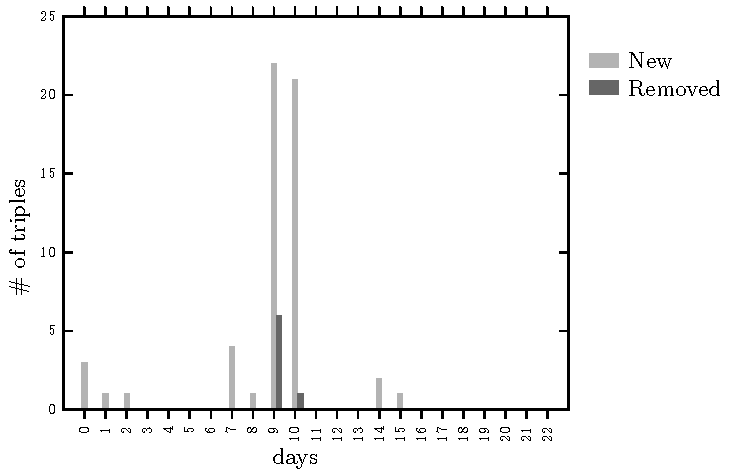
\includegraphics[width=0.8\textwidth]{images/updating_1.pdf}
  \end{center}
  \caption{Number of new coming soon movies, which are published on IMDb per day.}
  \label{fig_coming_soon_movie}
\end{figure}

In Figure \ref{fig_new_movie}, the number of changed triples of a newly released movie from IMDb is displayed.
Therefor, the movie was crawled and triplified daily.
As you can seen, the movie frequently changes in the first days.
Some triples which are changing often are cast triple, links to images and videos, IMDb rating, character triples or taglines.

\begin{figure}[h!]
  \begin{center}
  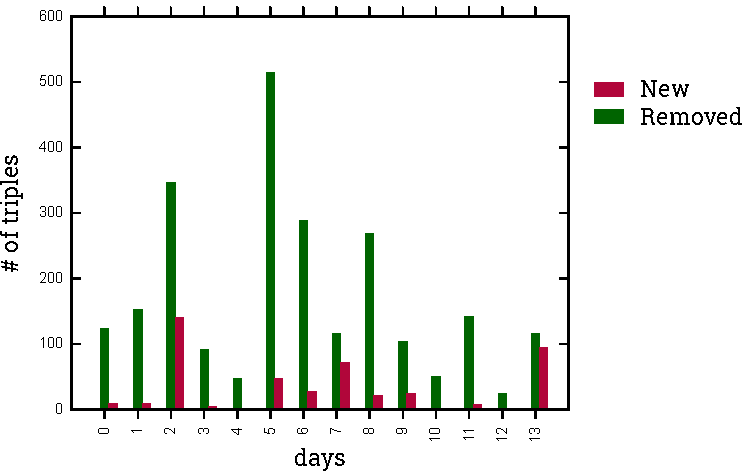
\includegraphics[width=0.8\textwidth]{images/updating_2.pdf}
  \end{center}
  \caption{Number of triples, which change in the first days of a new released movie from IMDb.}
  \label{fig_new_movie}
\end{figure}